% Fig. 1: depot system. Compile: pdflatex fig1_depot.tex  (standalone, output copied to ../fig1_depot.pdf)
\documentclass[tikz,border=2pt]{standalone}
\usepackage{mathptmx}
\usetikzlibrary{arrows.meta,positioning,fit,calc,backgrounds}
\definecolor{ink}{HTML}{1F1F1F}
\definecolor{ink2}{HTML}{555555}
\definecolor{blu}{HTML}{2A78D6}
\definecolor{blul}{HTML}{CDE2FB}
\definecolor{grn}{HTML}{1BAF7A}
\definecolor{yel}{HTML}{EDA100}
\definecolor{red}{HTML}{E34948}
\definecolor{gry}{HTML}{F0F0F0}
\begin{document}
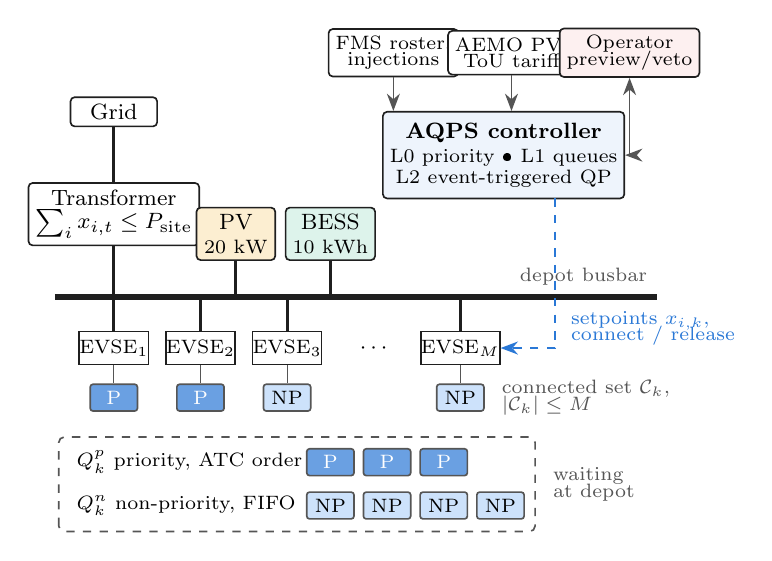
\begin{tikzpicture}[
  font=\footnotesize, >={Stealth[length=2.2mm]}, line width=0.6pt, draw=ink,
  box/.style={draw=ink, rounded corners=1.5pt, align=center, inner sep=2.5pt, fill=white},
  evse/.style={draw=ink, fill=white, minimum width=7mm, minimum height=4.2mm, inner sep=0pt, font=\scriptsize},
  ev/.style={draw=ink2, rounded corners=1pt, minimum width=6mm, minimum height=3.4mm, inner sep=0pt, font=\scriptsize},
  pw/.style={-, line width=1.1pt, draw=ink},
  ctl/.style={->, draw=blu, dashed, line width=0.7pt},
  dat/.style={->, draw=ink2, line width=0.6pt},
]
% ---------------- power side
\node[box, minimum width=11mm] (grid) at (0,4.75) {Grid};
\node[box] (tx) at (0,3.45) {Transformer\\[-1pt]$\textstyle\sum_i x_{i,t}\le P_\mathrm{site}$};
\draw[pw] (grid) -- (tx);
\draw[pw] (tx.south) -- (0,2.4);
\draw[line width=2.2pt, draw=ink] (-0.75,2.4) -- (6.9,2.4);
\node[font=\scriptsize, ink2, anchor=south east] at (6.9,2.42) {depot busbar};
\node[box, fill=yel!18, minimum width=10mm] (pv) at (1.55,3.2) {PV\\[-1pt]\scriptsize 20 kW};
\node[box, fill=grn!15, minimum width=10mm] (bess) at (2.75,3.2) {BESS\\[-1pt]\scriptsize 10 kWh};
\draw[pw] (pv.south) -- (1.55,2.4);
\draw[pw] (bess.south) -- (2.75,2.4);
\foreach \k/\x/\lab in {0/0/1, 1/1.1/2, 2/2.2/3, 4/4.4/M} {
  \node[evse] (e\k) at (\x,1.75) {EVSE$_{\lab}$};
  \draw[pw] (e\k.north) -- (\x,2.4);
}
\node at (3.3,1.75) {$\cdots$};
\node[ev, fill=blu!70, text=white] (c0) at (0,1.12) {P};
\node[ev, fill=blu!70, text=white] (c1) at (1.1,1.12) {P};
\node[ev, fill=blul] (c2) at (2.2,1.12) {NP};
\node[ev, fill=blul] (c4) at (4.4,1.12) {NP};
\foreach \k in {0,1,2,4} {\draw[ink2, line width=0.4pt] (e\k.south) -- (c\k.north);}
\node[font=\scriptsize, ink2, anchor=west, align=left] at (4.8,1.12) {connected set $\mathcal{C}_k$,\\[-2pt]$|\mathcal{C}_k|\le M$};
% waiting queues
\node[font=\scriptsize, anchor=west] (qp) at (-0.6,0.3) {$Q^{p}_k$ priority, ATC order};
\node[font=\scriptsize, anchor=west] (qn) at (-0.6,-0.25) {$Q^{n}_k$ non-priority, FIFO};
\foreach \j in {0,1,2} {\node[ev, fill=blu!70, text=white] at (2.75+0.72*\j,0.3) {P};}
\foreach \j in {0,1,2,3} {\node[ev, fill=blul] at (2.75+0.72*\j,-0.25) {NP};}
\draw[draw=ink2, dashed, rounded corners=2pt] (-0.7,-0.58) rectangle (5.35,0.62);
\node[font=\scriptsize, ink2, anchor=west, align=left] at (5.45,0.02) {waiting\\[-2pt]at depot};
% ---------------- control side
\node[box, fill=blu!8, minimum width=27mm, minimum height=11mm] (aqps) at (4.95,4.2)
  {\textbf{AQPS controller}\\[-1pt]\scriptsize L0 priority \textbullet\ L1 queues\\[-2pt]\scriptsize L2 event-triggered QP};
\node[box, font=\scriptsize] (fms) at (3.55,5.5) {FMS roster,\\[-2pt] injections};
\node[box, font=\scriptsize] (fc) at (5.05,5.5) {AEMO PV,\\[-2pt] ToU tariff};
\node[box, font=\scriptsize, fill=red!8] (op) at (6.55,5.5) {Operator\\[-2pt]preview/veto};
\draw[dat] (fms.south) -- (fms.south |- aqps.north);
\draw[dat] (fc.south) -- (fc.south |- aqps.north);
\draw[<->, draw=ink2, line width=0.6pt] (op.south) |- (aqps.east);
\draw[ctl] (5.6,3.65) -- (5.6,1.75) -- (e4.east);
\node[font=\scriptsize, blu, anchor=west, align=left] at (5.68,2.0) {setpoints $x_{i,k}$,\\[-2pt]connect / release};
\end{tikzpicture}
\end{document}
